% !TEX TS-program = pdflatex
% !TEX encoding = UTF-8 Unicode

% This is a simple template for a LaTeX document using the "article" class.
% See "book", "report", "letter" for other types of document.

\documentclass[11pt]{article} % use larger type; default would be 10pt

\usepackage[utf8]{inputenc} % set input encoding (not needed with XeLaTeX)
\usepackage{tikz}
%%% Examples of Article customizations
% These packages are optional, depending whether you want the features they provide.
% See the LaTeX Companion or other references for full information.

%%% PAGE DIMENSIONS
\usepackage{geometry} % to change the page dimensions
\geometry{a4paper} % or letterpaper (US) or a5paper or....
% \geometry{margins=2in} % for example, change the margins to 2 inches all round
% \geometry{landscape} % set up the page for landscape
%   read geometry.pdf for detailed page layout information

\usepackage{graphicx} % support the \includegraphics command and options

% \usepackage[parfill]{parskip} % Activate to begin paragraphs with an empty line rather than an indent

%%% PACKAGES
\usepackage{booktabs} % for much better looking tables
\usepackage{array} % for better arrays (eg matrices) in maths
\usepackage{paralist} % very flexible & customisable lists (eg. enumerate/itemize, etc.)
\usepackage{verbatim} % adds environment for commenting out blocks of text & for better verbatim
\usepackage{subfig} % make it possible to include more than one captioned figure/table in a single float
% These packages are all incorporated in the memoir class to one degree or another...
\usepackage{url}
\usepackage{hyperref}

%%% HEADERS & FOOTERS
\usepackage{fancyhdr} % This should be set AFTER setting up the page geometry
\pagestyle{fancy} % options: empty , plain , fancy
\renewcommand{\headrulewidth}{0pt} % customise the layout...
\lhead{}\chead{}\rhead{}
\lfoot{}\cfoot{\thepage}\rfoot{}

%%% SECTION TITLE APPEARANCE
\usepackage{sectsty}
\allsectionsfont{\sffamily\mdseries\upshape} % (See the fntguide.pdf for font help)
% (This matches ConTeXt defaults)

%%% ToC (table of contents) APPEARANCE
\usepackage[nottoc,notlof,notlot]{tocbibind} % Put the bibliography in the ToC
\usepackage[titles,subfigure]{tocloft} % Alter the style of the Table of Contents
\renewcommand{\cftsecfont}{\rmfamily\mdseries\upshape}
\renewcommand{\cftsecpagefont}{\rmfamily\mdseries\upshape} % No bold!

%%% END Article customizations

%%% The "real" document content comes below...

\usepackage{amsfonts}
\usepackage{amsmath}
\usepackage{amsthm}
\usepackage{amssymb}
\usepackage{wasysym}

\theoremstyle{definition}
\newtheorem*{beispiel}{Beispiel}
\newtheorem{definition}{Definition}
\newtheorem*{bemerkung}{Bemerkung}
\newtheorem*{beweis}{Beweis}
\newtheorem*{ubung}{Übung}

\title{Selbststudium 5}
\author{Florian Lüthi}
%\date{} % Activate to display a given date or no date (if empty),
         % otherwise the current date is printed 

\begin{document}
\maketitle

\section*{Aufgabe 6.2.6a)}

Zeichnen wir zuerst einmal $P$:

\begin{center}
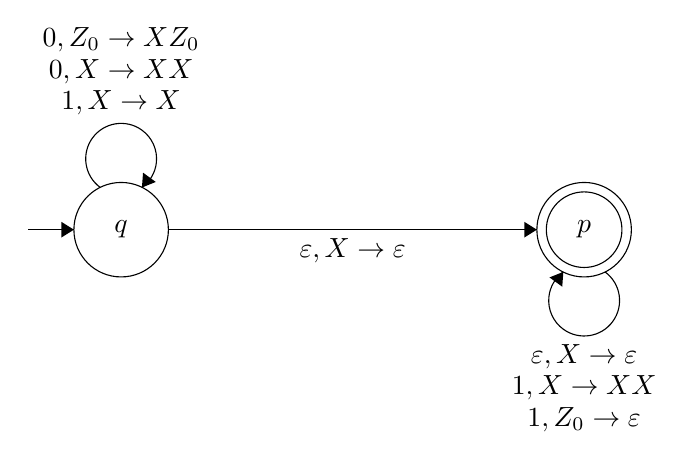
\begin{tikzpicture}[scale=0.2]
\tikzstyle{every node}+=[inner sep=0pt]
\draw [black] (23.2,-32.3) circle (3);
\draw (23.2,-32.3) node {$q$};
\draw [black] (52.6,-32.3) circle (3);
\draw (52.6,-32.3) node {$p$};
\draw [black] (52.6,-32.3) circle (2.4);
\draw [black] (17.3,-32.3) -- (20.2,-32.3);
\fill [black] (20.2,-32.3) -- (19.4,-31.8) -- (19.4,-32.8);
\draw [black] (21.877,-29.62) arc (234:-54:2.25);
\draw (23.2,-21.05) node [above] {$0,Z_0\rightarrow XZ_0$};
\draw (23.2,-23.05) node [above] {$0,X\rightarrow XX$};
\draw (23.2,-25.05) node [above] {$1,X\rightarrow X$};
\fill [black] (24.52,-29.62) -- (25.4,-29.27) -- (24.59,-28.68);
\draw [black] (26.2,-32.3) -- (49.6,-32.3);
\fill [black] (49.6,-32.3) -- (48.8,-31.8) -- (48.8,-32.8);
\draw (37.9,-32.8) node [below] {$\varepsilon,X\rightarrow\varepsilon$};
\draw [black] (53.923,-34.98) arc (54:-234:2.25);
\draw (52.6,-39.55) node [below] {$\varepsilon,X\rightarrow\varepsilon$};
\draw (52.6,-41.55) node [below] {$1,X\rightarrow XX$};
\draw (52.6,-43.55) node [below] {$1,Z_0\rightarrow\varepsilon$};
\fill [black] (51.28,-34.98) -- (50.4,-35.33) -- (51.21,-35.92);
\end{tikzpicture}
\end{center}

Erfinden wir nun die Stackanfangsmarkierung $X_0$ (gleichzeitig das Startsymbol von $P_1$), einen neuen Startzustand $p_0$, einen nur durch Stackentleerung erreichbaren Zustand $f$ sowie die entsprechenden $\varepsilon$-Übergänge:

\begin{center}
\begin{tikzpicture}[scale=0.2]
\tikzstyle{every node}+=[inner sep=0pt]
\draw [black] (30.3,-32.3) circle (3);
\draw (30.3,-32.3) node {$q$};
\draw [black] (52.6,-32.3) circle (3);
\draw (52.6,-32.3) node {$p$};
\draw [black] (10.1,-32.3) circle (3);
\draw (10.1,-32.3) node {$p_0$};
\draw [black] (52.6,-17.6) circle (3);
\draw (52.6,-17.6) node {$f$};
\draw [black] (28.977,-29.62) arc (234:-54:2.25);
\draw (30.3,-21.05) node [above] {$0,Z_0\rightarrow XZ_0$};
\draw (30.3,-23.05) node [above] {$0,X\rightarrow XX$};
\draw (30.3,-25.05) node [above] {$1,X\rightarrow X$};
\fill [black] (31.62,-29.62) -- (32.5,-29.27) -- (31.69,-28.68);
\draw [black] (33.3,-32.3) -- (49.6,-32.3);
\fill [black] (49.6,-32.3) -- (48.8,-31.8) -- (48.8,-32.8);
\draw (41.45,-32.8) node [below] {$\varepsilon,X\rightarrow \varepsilon$};
\draw [black] (53.923,-34.98) arc (54:-234:2.25);
\draw (52.6,-39.55) node [below] {$\varepsilon,X\rightarrow \varepsilon$};
\draw (52.6,-41.55) node [below] {$1,X \rightarrow XX$};
\draw (52.6,-43.55) node [below] {$1,Z_0 \rightarrow \varepsilon$};
\fill [black] (51.28,-34.98) -- (50.4,-35.33) -- (51.21,-35.92);
\draw [black] (3.5,-32.3) -- (7.1,-32.3);
\fill [black] (7.1,-32.3) -- (6.3,-31.8) -- (6.3,-32.8);
\draw [black] (13.1,-32.3) -- (27.3,-32.3);
\fill [black] (27.3,-32.3) -- (26.5,-31.8) -- (26.5,-32.8);
\draw (20.2,-32.8) node [below] {$\varepsilon,X_0\rightarrow Z_0X_0$};
\draw [black] (52.6,-29.3) -- (52.6,-20.6);
\fill [black] (52.6,-20.6) -- (52.1,-21.4) -- (53.1,-21.4);
\draw (53.1,-24.95) node [right] {$\varepsilon,\textrm{beliebig}\rightarrow\varepsilon$};
\draw [black] (51.277,-14.92) arc (234:-54:2.25);
\draw (52.6,-10.35) node [above] {$\varepsilon,\textrm{beliebig}\rightarrow \varepsilon$};
\fill [black] (53.92,-14.92) -- (54.8,-14.57) -- (53.99,-13.98);
\end{tikzpicture}
\end{center}

Und dadurch haben wir nun \[
P_1 = (\{ p_0, q, p, f \}, \{0,1\}, \{X_0, Z_0, X\}, \delta, p_0, X_0)
\]
mit $\delta$ gemäss obiger Zeichnung gefunden. Es gilt $N(P_1) = L(P)$.

\section*{Aufgabe 6.2.6b)}

Zeichnen wir wiederum $P$, diesmal als durch Stackentleerung akzeptierenden PDA:

\begin{center}
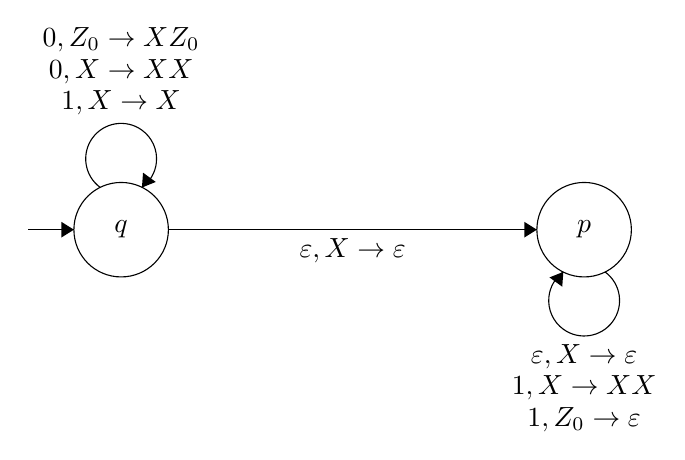
\begin{tikzpicture}[scale=0.2]
\tikzstyle{every node}+=[inner sep=0pt]
\draw [black] (23.2,-32.3) circle (3);
\draw (23.2,-32.3) node {$q$};
\draw [black] (52.6,-32.3) circle (3);
\draw (52.6,-32.3) node {$p$};
\draw [black] (17.3,-32.3) -- (20.2,-32.3);
\fill [black] (20.2,-32.3) -- (19.4,-31.8) -- (19.4,-32.8);
\draw [black] (21.877,-29.62) arc (234:-54:2.25);
\draw (23.2,-21.05) node [above] {$0,Z_0\rightarrow XZ_0$};
\draw (23.2,-23.05) node [above] {$0,X\rightarrow XX$};
\draw (23.2,-25.05) node [above] {$1,X\rightarrow X$};
\fill [black] (24.52,-29.62) -- (25.4,-29.27) -- (24.59,-28.68);
\draw [black] (26.2,-32.3) -- (49.6,-32.3);
\fill [black] (49.6,-32.3) -- (48.8,-31.8) -- (48.8,-32.8);
\draw (37.9,-32.8) node [below] {$\varepsilon,X\rightarrow\varepsilon$};
\draw [black] (53.923,-34.98) arc (54:-234:2.25);
\draw (52.6,-39.55) node [below] {$\varepsilon,X\rightarrow\varepsilon$};
\draw (52.6,-41.55) node [below] {$1,X\rightarrow XX$};
\draw (52.6,-43.55) node [below] {$1,Z_0\rightarrow\varepsilon$};
\fill [black] (51.28,-34.98) -- (50.4,-35.33) -- (51.21,-35.92);
\end{tikzpicture}
\end{center}

Erfinden wir einen neuen Startzustand $p_0$, ein Markierungssymbol $X_0$, einen neuen finalen Zustand $f$ sowie die entsprechenden $\varepsilon$-Übergänge:

\begin{center}
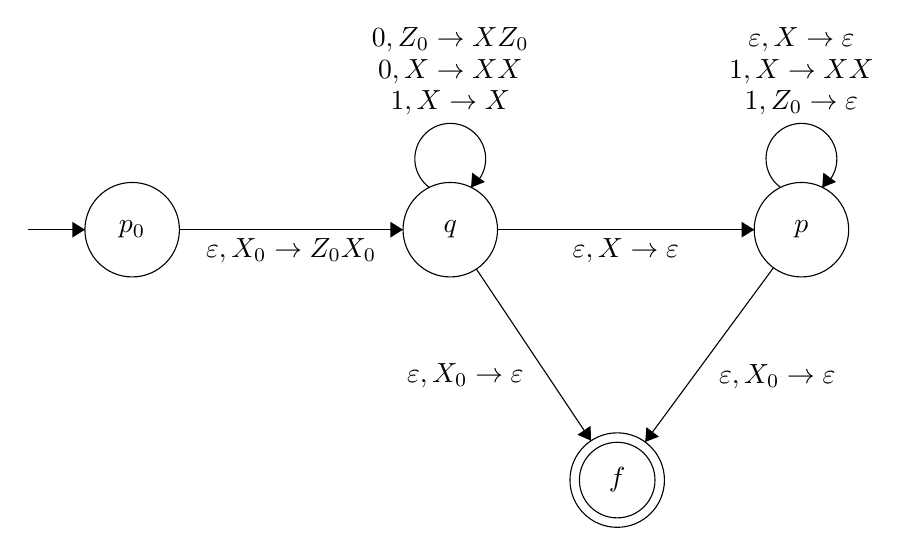
\begin{tikzpicture}[scale=0.2]
\tikzstyle{every node}+=[inner sep=0pt]
\draw [black] (30.3,-32.3) circle (3);
\draw (30.3,-32.3) node {$q$};
\draw [black] (52.6,-32.3) circle (3);
\draw (52.6,-32.3) node {$p$};
\draw [black] (10.1,-32.3) circle (3);
\draw (10.1,-32.3) node {$p_0$};
\draw [black] (40.9,-48.2) circle (3);
\draw (40.9,-48.2) node {$f$};
\draw [black] (40.9,-48.2) circle (2.4);
\draw [black] (28.977,-29.62) arc (234:-54:2.25);
\draw (30.3,-21.05) node [above] {$0,Z_0\rightarrow XZ_0$};
\draw (30.3,-23.05) node [above] {$0,X\rightarrow XX$};
\draw (30.3,-25.05) node [above] {$1,X\rightarrow X$};
\fill [black] (31.62,-29.62) -- (32.5,-29.27) -- (31.69,-28.68);
\draw [black] (33.3,-32.3) -- (49.6,-32.3);
\fill [black] (49.6,-32.3) -- (48.8,-31.8) -- (48.8,-32.8);
\draw (41.45,-32.8) node [below] {$\varepsilon,X\rightarrow \varepsilon$};
\draw [black] (51.277,-29.62) arc (234:-54:2.25);
\draw (52.6,-21.05) node [above] {$\varepsilon,X\rightarrow \varepsilon$};
\draw (52.6,-23.05) node [above] {$1,X \rightarrow XX$};
\draw (52.6,-25.05) node [above] {$1,Z_0 \rightarrow \varepsilon$};
\fill [black] (53.92,-29.62) -- (54.8,-29.27) -- (53.99,-28.68);
\draw [black] (3.5,-32.3) -- (7.1,-32.3);
\fill [black] (7.1,-32.3) -- (6.3,-31.8) -- (6.3,-32.8);
\draw [black] (13.1,-32.3) -- (27.3,-32.3);
\fill [black] (27.3,-32.3) -- (26.5,-31.8) -- (26.5,-32.8);
\draw (20.2,-32.8) node [below] {$\varepsilon,X_0\rightarrow Z_0X_0$};
\draw [black] (50.82,-34.72) -- (42.68,-45.78);
\fill [black] (42.68,-45.78) -- (43.55,-45.44) -- (42.75,-44.84);
\draw (47.33,-41.64) node [right] {$\varepsilon,X_0\rightarrow \varepsilon$};
%\draw [black] (42.223,-50.88) arc (54:-234:2.25);
%\fill [black] (39.58,-50.88) -- (38.7,-51.23) -- (39.51,-51.82);
\draw [black] (31.96,-34.8) -- (39.24,-45.7);
\fill [black] (39.24,-45.7) -- (39.21,-44.76) -- (38.38,-45.32);
\draw (34.99,-41.58) node [left] {$\varepsilon,X_0\rightarrow\varepsilon$};
\end{tikzpicture}
\end{center}

Und dadurch haben wir nun \[
P_2 = (\{ p_0, q, p, f \}, \{0,1\}, \{X_0, Z_0, X\}, \delta, p_0, X_0)
\]
mit $\delta$ gemäss obiger Zeichnung gefunden. Es gilt $L(P_2) = N(P)$.


\end{document}
